% =====================================================================
% Manual técnico
% Responsable: Parte 5 — Óscar Iván Ulises Gutiérrez Palacios
% =====================================================================
\section{Manual técnico}
\label{sec:manual-tecnico}

Este manual describe la solución desde el punto de vista de su construcción y de su
funcionamiento interno. Está dirigido a quien necesite instalar el entorno, comprender
cómo está organizado el programa y reproducir los experimentos, o bien extenderlo: un
resultado de simulación solo es confiable si otra persona puede volver a obtenerlo.

\subsection{Requisitos del sistema}

El entorno de referencia del grupo es Ubuntu 22.04 LTS, en ejecución nativa o mediante
WSL2 sobre Windows, que es la configuración con la que se documentó la instalación y se
corrieron los experimentos. El programa no depende de esa distribución en particular:
también puede ejecutarse en Windows nativo o en otras distribuciones de Linux, siempre
que se disponga de los programas y librerías que se indican a continuación.

\subsection{Programas y librerías necesarios}

Se requiere lo siguiente:

\begin{itemize}
    \item ns-3.43, con los módulos \texttt{wifi}, \texttt{aodv}, \texttt{mobility},
    \texttt{internet}, \texttt{applications} y \texttt{flow-monitor}. El módulo
    \texttt{netanim} es opcional y solo se usa para las trazas de visualización.
    \item Compilador de C++ compatible con C++17: GCC 11 o superior, Clang, o MSVC en
    Windows.
    \item CMake 3.22 o superior y Ninja.
    \item Python 3.10 o superior, requerido por el lanzador de ns-3.
    \item \texttt{wget} o \texttt{curl} con \texttt{bzip2} para descargar y descomprimir
    el paquete de ns-3.
\end{itemize}

La instalación de ns-3 se hace con la guía oficial de la plataforma elegida; una vez
instalado, el lanzador de ns-3 compila y ejecuta el programa con CMake y Ninja.

\subsection{Archivo fuente}

La simulación se entrega en un único archivo fuente, \texttt{manet-jerarquica.cc}. ns-3
solo compila los programas ubicados en su carpeta \texttt{scratch/}, así que ese archivo
se copia allí antes de ejecutar. Cada corrida escribe su XML de FlowMonitor y su resumen
en la carpeta de salida que se indique.

\subsection{Arquitectura del programa}

El programa está organizado en dos estructuras de datos y un conjunto de funciones, cada
una responsable de una fase de la simulación. La estructura \texttt{Parametros} reúne
todas las variables configurables por línea de comandos, desde el nombre del escenario y
las velocidades de movilidad hasta los alcances de radio y el directorio de salida. La
estructura \texttt{RedJerarquica} actúa como la interfaz compartida entre las fases:
guarda los contenedores de nodos agrupados por clúster y superclúster, la lista de
\emph{cluster heads}, la de miembros y las interfaces IP de cada subred.

Las funciones siguen el orden natural de construcción de la red. \texttt{CrearNodos}
instancia los veinte nodos y los agrupa; \texttt{ConfigurarRed} instala los canales WiFi,
la pila IP y el protocolo AODV, y asigna las subredes; \texttt{ConfigurarMovilidad}
monta la movilidad jerárquica en tres capas; \texttt{ConfigurarTrafico} inyecta los ocho
flujos UDP; y \texttt{ConfigurarMetricas} instala el monitor de flujos. Al terminar la
ejecución, \texttt{GuardarMetricas} serializa los resultados. La figura~\ref{fig:mt-arquitectura}
muestra la red que construyen esas funciones y la
figura~\ref{fig:mt-flujo} el orden en que se invocan.

\begin{figure}[h]
\centering
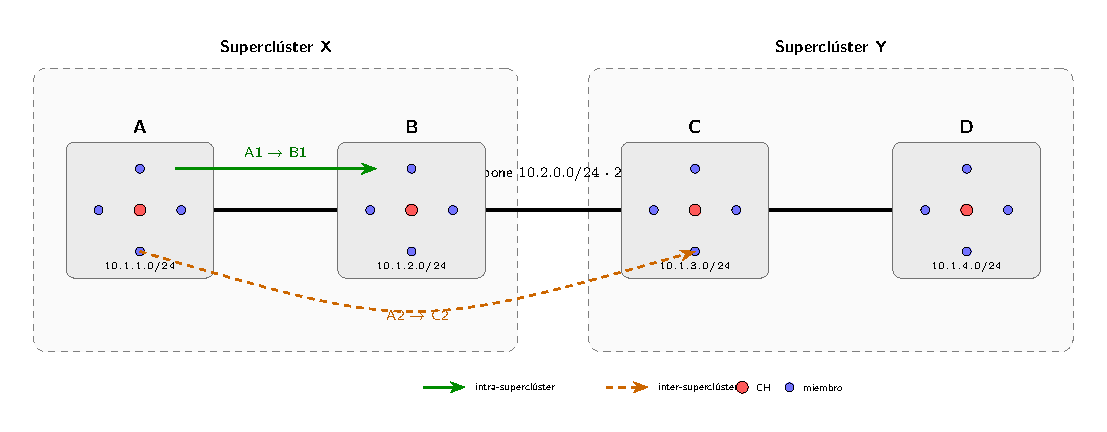
\includegraphics[width=0.9\textwidth]{Materiales/diagramas/arquitectura.pdf}
\caption{Arquitectura jerárquica construida por el programa: cuatro clústeres con su
canal propio y un \emph{backbone} compartido entre los \emph{cluster heads}.}
\label{fig:mt-arquitectura}
\end{figure}

\begin{figure}[h]
\centering
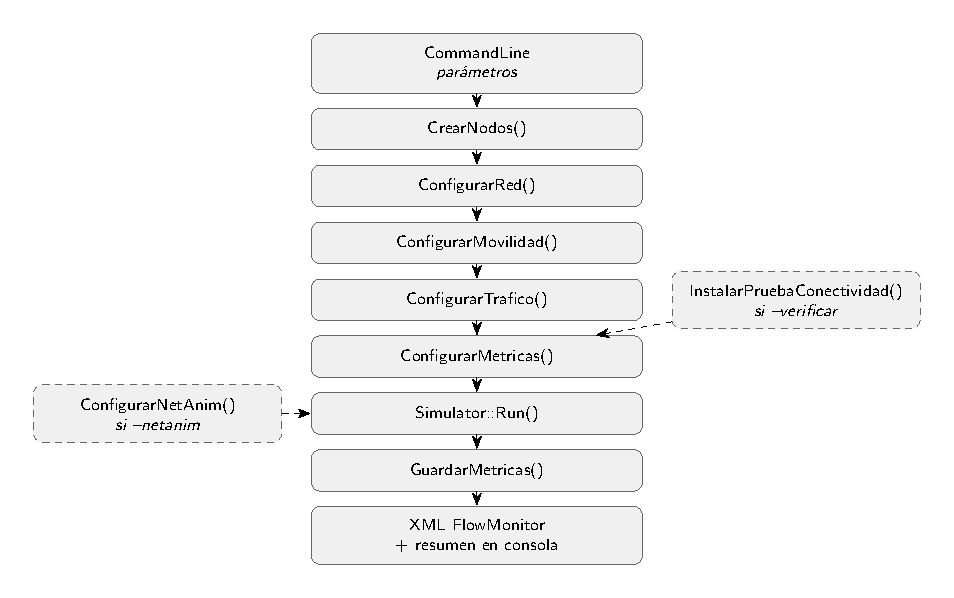
\includegraphics[width=0.8\textwidth]{Materiales/diagramas/flujo-simulacion.pdf}
\caption{Secuencia de fases de la simulación y correspondencia con las funciones del
programa.}
\label{fig:mt-flujo}
\end{figure}

\subsection{Configuración de red y movilidad}

La red separa la comunicación local de la comunicación interclúster. Cada clúster usa un
canal WiFi ad hoc independiente con un alcance efectivo de 60\,m, y los cuatro
\emph{cluster heads} comparten un canal \emph{backbone} con un alcance de 250\,m. La
propagación se modela con un disco de alcance exacto, de modo que un receptor recibe la
señal si y solo si su distancia al transmisor no supera el alcance configurado. El
direccionamiento asigna una subred por clúster ($10.1.1.0/24$ a $10.1.4.0/24$) y una
para el \emph{backbone} ($10.2.0.0/24$), y AODV corre sobre todas las interfaces.

La movilidad se compone con tres capas anidadas. El superclúster permanece fijo; el
clúster se mueve con un modelo \emph{Random Waypoint} de velocidad constante dentro de
una región de $\pm 150$\,m; y cada miembro se mueve con una caminata aleatoria
bidimensional dentro de una región de $\pm 40$\,m. Poner la velocidad de una capa en cero
equivale a dejarla quieta, que es exactamente como se aíslan los efectos en los
escenarios del experimento. Las velocidades son constantes, no un rango, para que los
escenarios sean comparables entre sí.

\subsection{Tráfico y métricas}

El tráfico consiste en ocho flujos UDP de tasa constante, con paquetes de 512 bytes a 4
paquetes por segundo (16\,kbit/s por flujo). Cuatro flujos comunican miembros de
clústeres del mismo superclúster y cuatro comunican miembros de superclústeres
distintos, de forma que todos los paquetes cruzan la jerarquía. Los flujos inician con
un desfase uniforme entre los 10 y los 11 segundos, para dejar que AODV estabilice sus
rutas, y terminan a los 195 segundos. Las métricas se obtienen con el módulo
\texttt{flow-monitor}, que por cada flujo contabiliza paquetes transmitidos y recibidos,
bytes, retardos y variación de retardo; a partir de esos contadores se calculan la tasa
de entrega, el retardo medio, el \emph{throughput} y el \emph{jitter}. El resultado se
guarda en un XML cuyo nombre codifica el escenario, las velocidades y la réplica, con el
formato \texttt{<escenario>\_cs<clusterSpeed>\_ns<nodeSpeed>\_run<RngRun>.xml}.

\subsection{Ejecución del programa}

Para ejecutar una simulación se copia el programa a la carpeta \texttt{scratch/} de ns-3
y se invoca el lanzador con los parámetros deseados:

\begin{verbatim}
cp manet-jerarquica.cc \
    ~/ns-allinone-3.43/ns-3.43/scratch/
cd ~/ns-allinone-3.43/ns-3.43
./ns3 run "scratch/manet-jerarquica --scenario=E3 --clusterSpeed=5 \
    --nodeSpeed=5 --simTime=200 --RngRun=1"
\end{verbatim}

La primera ejecución compila el programa; las siguientes lo reutilizan. El nombre del
escenario es solo una etiqueta: lo que determina qué se mueve son las velocidades. El
programa imprime al inicio la topología y, al final, un resumen con los totales
agregados. Ese resumen incluye también el tráfico de control de AODV, por lo que las
cifras que se calculan sobre los flujos de datos únicamente no coinciden con las de la
consola.


